\documentclass{beamer}
\usepackage[utf8]{inputenc}
\usepackage[T1]{fontenc}
\usepackage[english]{babel}
\usepackage{graphicx}
\usepackage{times}
\usepackage{adjustbox}
\usetheme{AGH}

\title{Akwizycja danych dla identyfikacji prostego modelu opad-odpływ}
\title[]{Akwizycja danych dla identyfikacji \\ prostego modelu opad-odpływ}

\author[F. Pasternak]{Filip Pasternak}

\date[2016]{25-01-2016}

\institute[AGH]
{Promotor: dr inż Janusz Miller \\ Wydział EAIiIB}

%\setbeamertemplate{itemize item}{$\maltese$}

\begin{document}

{
%\usebackgroundtemplate{
\includegraphics[width=\paperwidth]{titlepage}} % wersja angielska
\usebackgroundtemplate{
\includegraphics[width=\paperwidth]{titlepagepl}} % wersja polska
 \begin{frame}
   \titlepage
 \end{frame}
}


%---------------------------------------------------------------------------

%---------------------------------------------------------------------------

\begin{frame}
\frametitle{Plan prezentacji}
\begin{itemize}
\item{Cele pracy}
\item{Wprowadzenie teoretyczne}
\item{Implementacja rozwiązania}
\item{Uzyskane rezultaty}
\item{Podsumowanie}
\end{itemize}

\end{frame}

%---------------------------------------------------------------------------

\begin{frame}
\frametitle{Cele pracy}
\begin{itemize}
\item{Przegląd możliwości odczytu rzeczywistych danych opadowych i~wodowskazowych.}

\item{Stworzenie narzędzia dokonującego przetwarzania pomiarów z~posterunków opadowych, aby wyznaczyć objętość wody deszczowej jaka spadła na zadany obszar.}

\item{Przeprowadzenie analizy wpływu wykluczenia poszczególnych punktów opadowych na uzyskane wskazania.}


\end{itemize}
\end{frame}
%---------------------------------------------------------------------------
\begin{frame}
\frametitle{Metody wyznaczania opadu powierzchniowego}

Przykładowe metody powszechnie stosowane do wyznaczania opadu powierzchniowego:
\begin{itemize}
\item{Metoda Thiessena}
\item{Metoda izohiet}
\item{Metoda krzywej hipsometrycznej}
\item{Metoda regionów opadowych}
\end{itemize}

\end{frame}
%---------------------------------------------------------------------------

\begin{frame}
\frametitle{Zastosowana metoda}

Kroki zastosowanego algorytmu:
\begin{itemize}
	\item{Utworzenie, metodą triangulacji, siatki ze zbioru punktów opadowych.}
	\item{Wyznaczenie punktów przecięcia granicy zlewni z~krawędziami trójkątów siatki.}	
	\item{Interpolacja wartości opadu w~wyznaczonych punktach.}
	\item{Triangulacja zbioru punktów należących do obszaru zlewni.}
	\item{Wyznaczenie objętości opadu na powstałych trójkątach.}
	\item{Uzyskanie łącznej ilości wody opadowej na wskazanym obszarze.}
\end{itemize}
\end{frame}
%---------------------------------------------------------------------------

\begin{frame}
\frametitle{Implementacja rozwiązania}
\begin{itemize}
\item{Użyte zostało środowisko MatLab 2015b.}
\item{Triangulacja oparta o~klasę \textit{delaunayTriangulation}.}
\item{Brak dostępu do danych rzeczywistych IMGW.}
\item{Stworzono funkcje symulujące dane wejściowe na potrzeby projektu.}
\end{itemize}
\begin{minipage}[t]{\linewidth}
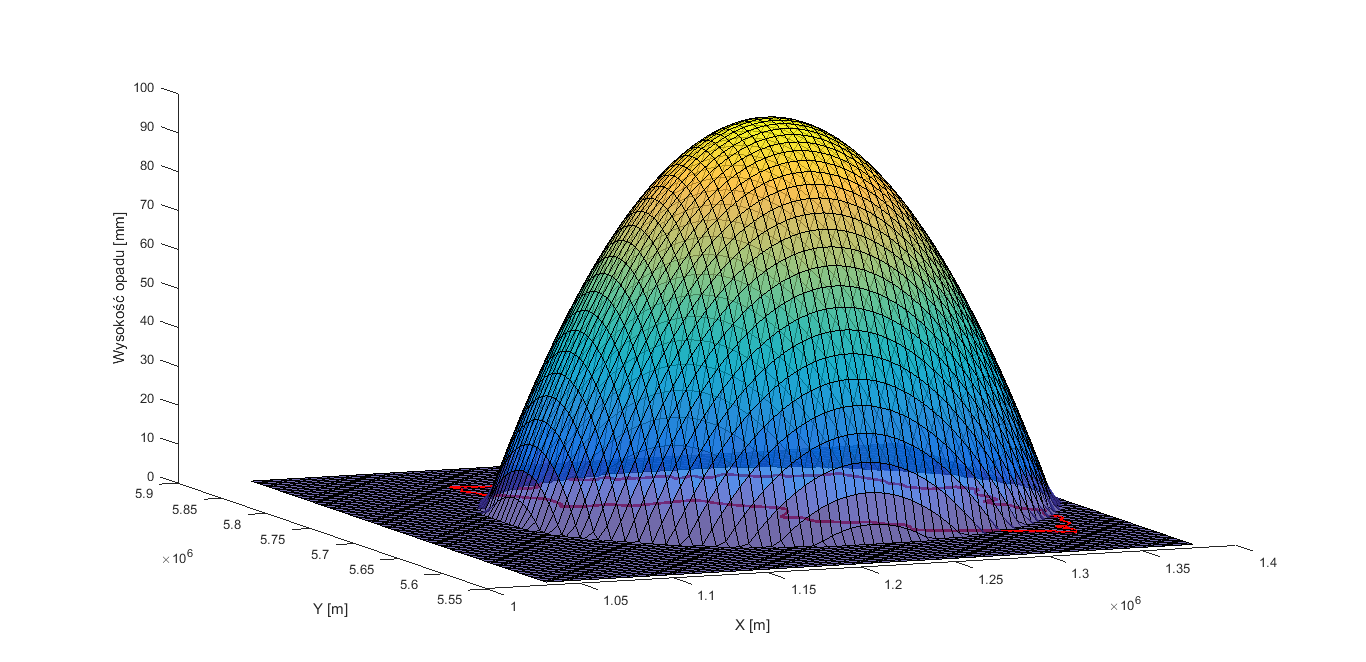
\includegraphics[width=.5\textwidth]{./../img/chmura_paraboloidalna_1.png}
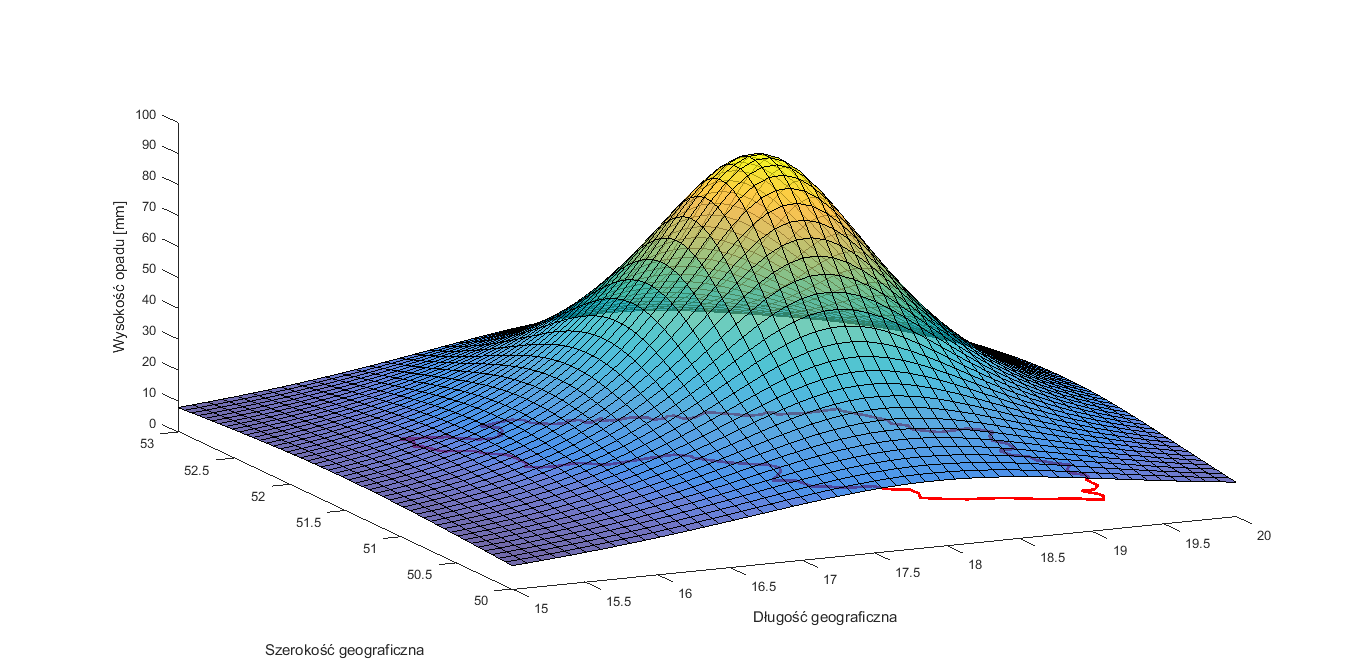
\includegraphics[width=.5\textwidth]{./../img/chmura_wymierna_1.png}
\end{minipage}

\end{frame}

%---------------------------------------------------------------------------

\begin{frame}
\frametitle{Implementacja - interpolacja opadu}
\begin{minipage}[t]{\linewidth}
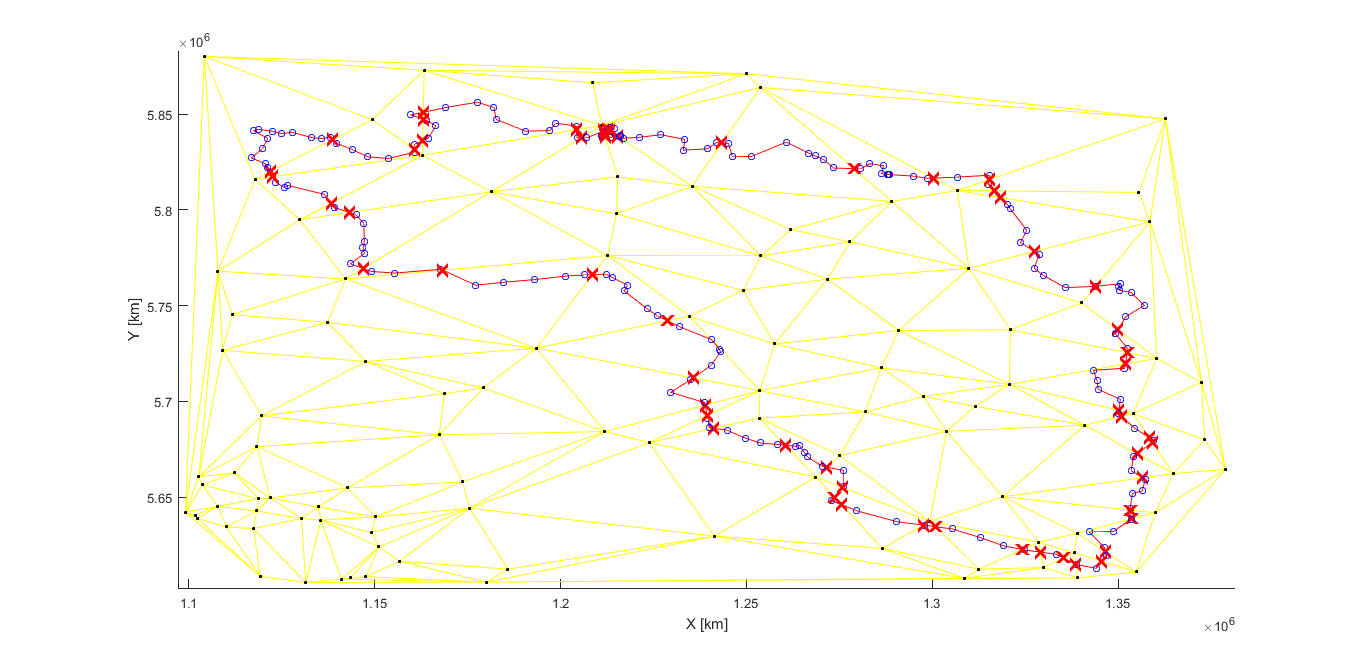
\includegraphics[width=.5\textwidth]{./../img/punkty_do_interpolacji.png}
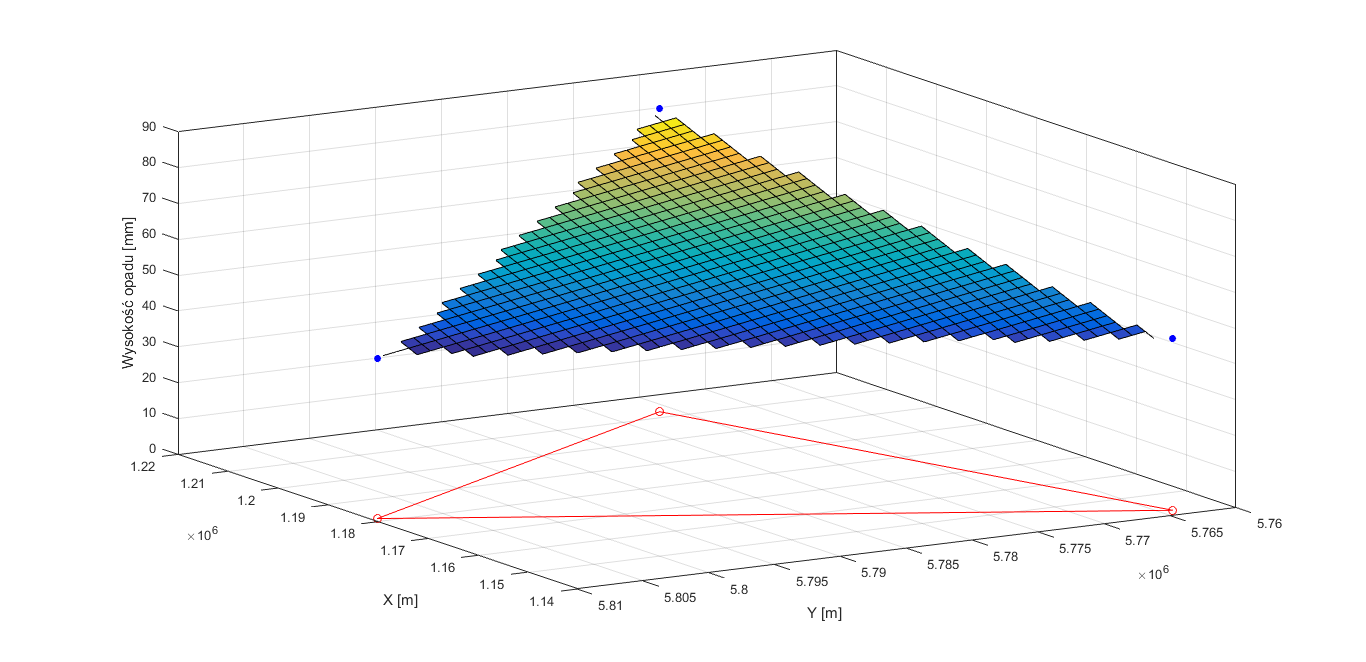
\includegraphics[width=.5\textwidth]{./../img/prezentacja_interpolacji.png}
\end{minipage}
\end{frame}
%---------------------------------------------------------------------------
\begin{frame}
\frametitle{Implementacja - podział zlewni}
\begin{minipage}[t]{\linewidth}
\centering
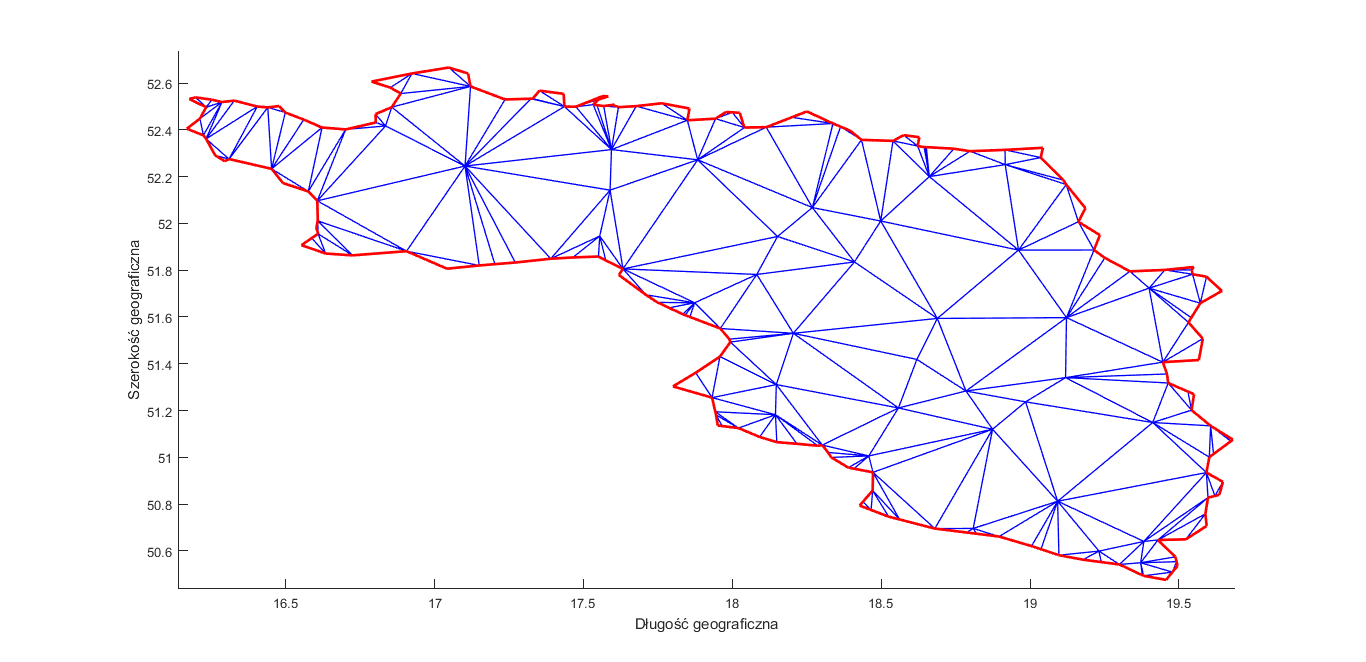
\includegraphics[width=.8\textwidth]{./../img/druga_triangulacja_z_ograniczeniem.png}
\end{minipage}
\end{frame}

%---------------------------------------------------------------------------

\begin{frame}
\frametitle{Wyniki - objętość opadu}
\begin{table}[!ht]
\begin{center}
\begin{tabular}{|c|c|c|}
\hline
 Wariant                 &  Paraboliczny      & Wymierny \\ \hline
Opad wyznaczony [$m^3$]  &  1 462 995 563.4253  & 1 559 081 843.8972 \\ \hline
Opad rzeczywisty [$m^3$] & 1 500 568 329.7155 & 1 571 689 381.8665 \\ \hline
Różnica [\%] & -2.5039 & -0.8022 \\ \hline
\end{tabular}
\end{center}
\end{table}
\end{frame}


%---------------------------------------------------------------------------
\begin{frame}
\frametitle{Wyniki - wpływ wykluczenia posterunku}
\begin{itemize}
\item{Wyłączenie punktów, takich jak 9 i 11, zmniejszyło dokładność wyniku.}
\item{Wyłączenie punktów, takich jak 8 i 17, nie wpłynęło na rezultat programu.}
\end{itemize}
%\begin{figure}
\centering
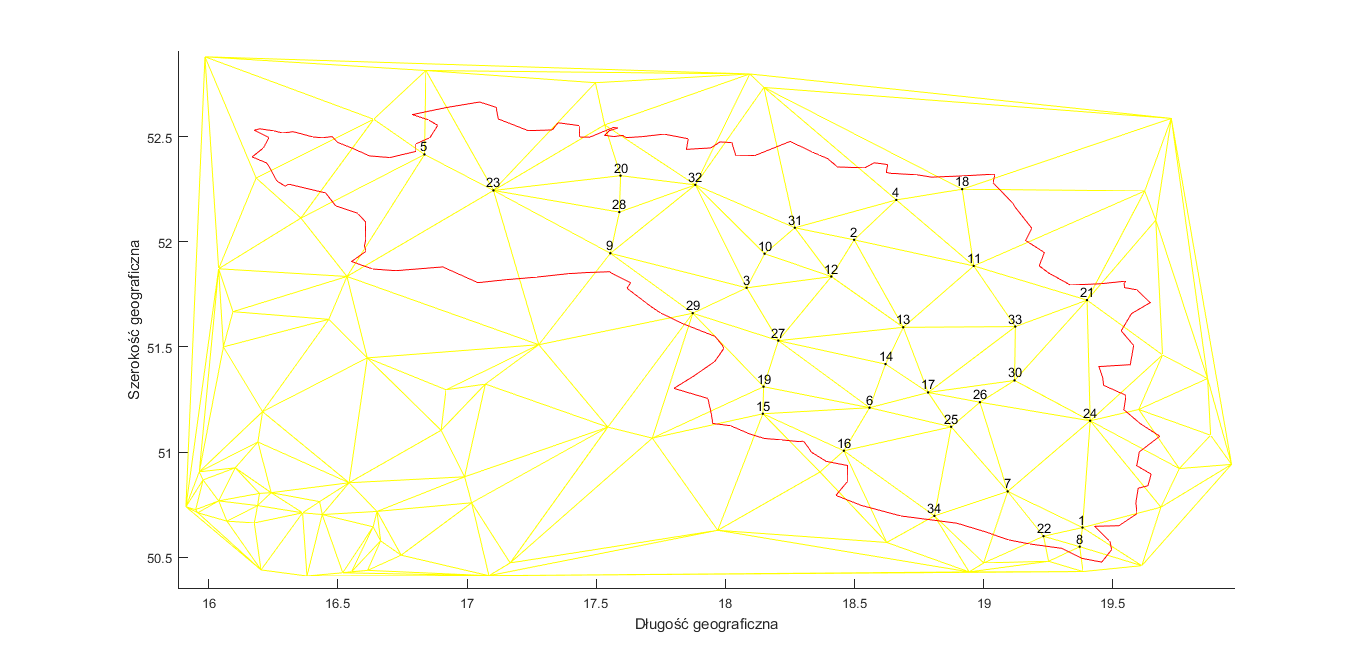
\includegraphics[width=.8\textwidth]{./../img/identyfikatory_punktow.png}
%\end{figure}

\end{frame}


%---------------------------------------------------------------------------
\begin{frame}
\frametitle{Podsumowanie}
\begin{itemize}
	\item{Utworzone narzędzie osiąga zadowalające wyniki.}
	\item{Istnieją możliwości rozszerzenia/usprawnienia narzędzia.}
	\item{Możliwość wdrożenia projektu jako składnika systemu ostrzegającego przed powodzią.}

\end{itemize}
\end{frame}



\end{document}
